\iffalse
\documentclass[12pt]{article}
\usepackage{graphicx}
%\documentclass[journal,12pt,twocolumn]{IEEEtran}
\usepackage[none]{hyphenat}
\usepackage{graphicx}
\usepackage{listings}
\usepackage[english]{babel}
\usepackage{graphicx}
\usepackage{caption} 
\usepackage{hyperref}
\usepackage{booktabs}
\usepackage{array}
\usepackage{amsmath}   % for having text in math mode

%Following 2 lines were added to remove the blank page at the beginning
\usepackage{atbegshi}% http://ctan.org/pkg/atbegshi
\AtBeginDocument{\AtBeginShipoutNext{\AtBeginShipoutDiscard}}
%


%New macro definitions
\newcommand{\mydet}[1]{\ensuremath{\begin{vmatrix}#1\end{vmatrix}}}
\providecommand{\brak}[1]{\ensuremath{\left(#1\right)}}
\providecommand{\norm}[1]{\left\lVert#1\right\rVert}
\newcommand{\solution}{\noindent \textbf{Solution: }}
\newcommand{\myvec}[1]{\ensuremath{\begin{pmatrix}#1\end{pmatrix}}}
\let\vec\mathbf

\begin{document}

\begin{center}
\title{\textbf{Area of a Traingle}}
\date{\vspace{-5ex}} %Not to print date automatically
\maketitle
\end{center}

\setcounter{page}{1}



\section{10$^{th}$ Maths - Chapter 7}

This is Problem-1 from Exercise 7.3

\begin{enumerate}
\item Find the area of the triangle whose vertices are :
	\fi
\begin{enumerate}
\item 
In this case, the area  is given by  
  \label{prop:10/7/3/1area2d}
  \begin{align}
    \label{eq:10/7/3/1area2d}
	\frac{1}{2}\norm{\brak{\vec{A}-\vec{B}} \times \brak{\vec{A}-\vec{C}}} \\
  \end{align}
  Since
  \begin{align}
	 \vec{A}-\vec{B} =  \myvec{
  2 \\
  3 \\
 } - \myvec{
  -1 \\
  0 \\
 } = \myvec{
 3 \\
 3 \\
 }
 \\
 \vec{A}-\vec{C} =  \myvec{
  2 \\
  3 \\
 } - \myvec{
  2 \\
  -4 \\
 } = \myvec{
 0 \\
 7 \\
 }
 \end{align}
 the desired area is given by 
 \iffalse
The value of the cross product of two vectors is given by
\begin{align}
  \label{eq:10/7/3/1det2d}
  \mydet{\vec{M}} &= \mydet{\vec{A} & \vec{B}} 
  \\
  &= \mydet{a_1 & b_1\\a_2 & b_2} = a_1b_2 - a_2 b_1
\end{align}

		Therefore, \eqref{eq:10/7/3/1area2d} equals \\
		\fi
\begin{align}
	\frac{1}{2}\mydet{3 & 0\\3 & 7}  
	&=	\frac{21}{2}
\end{align}
\iffalse
\begin{figure}[!h]
	\begin{center}
		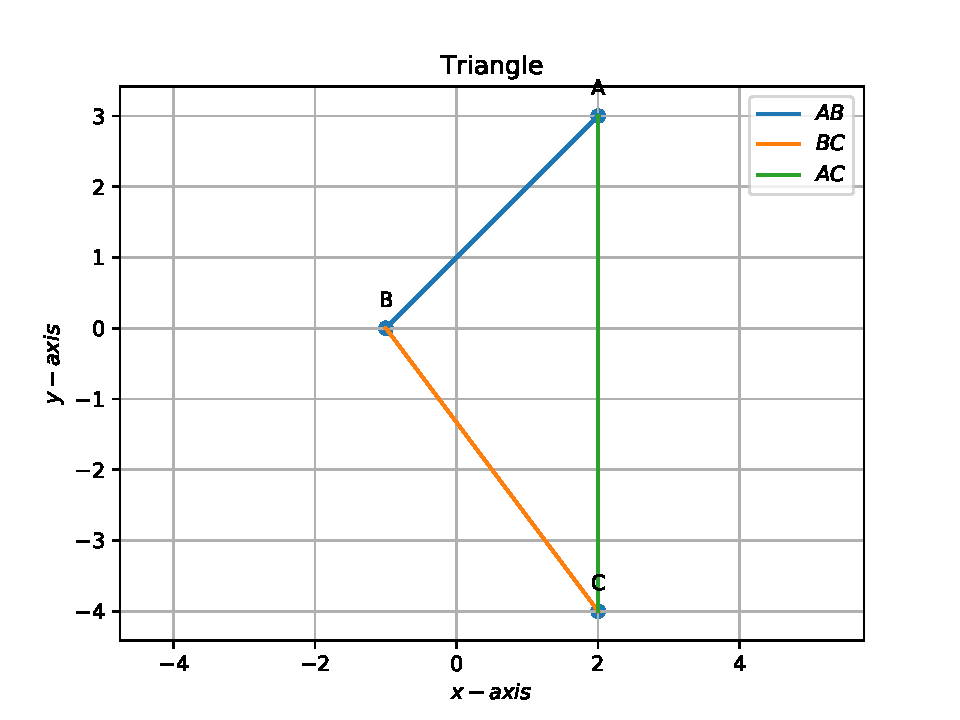
\includegraphics[width=\columnwidth]{./figs/problem1a.pdf}
	\end{center}
\caption{}
\label{fig:Fig1}
\end{figure}
\fi

\item In this case, 
	\iffalse
\solution The area of the triangle with vertices $\vec{A}, \vec{B}, \vec{C}$ is given by  
  \label{prop:10/7/3/1area2e}
  \begin{align}
    \label{eq:10/7/3/1area2e}
	\frac{1}{2}\norm{\brak{\vec{A}-\vec{B}} \times \brak{\vec{A}-\vec{C}}} \\
	\fi
  \begin{align}
	 \vec{A}-\vec{B} =  \myvec{
  -5 \\
  -1 \\
 } - \myvec{
  3 \\
  -5 \\
 } = \myvec{
 -8 \\
 4 \\
 }
 \\
 \vec{A}-\vec{C} =  \myvec{
  -5 \\
  -1 \\
 } - \myvec{
  5 \\
  2 \\
 } = \myvec{
 -10 \\
 -3 \\
 }
 \\
	  \implies
\text{Area} =	\frac{1}{2}\mydet{-8 & -10\\4 & -3}  
	=  32 
\end{align}
\iffalse
\begin{figure}[!h]
	\begin{center}
		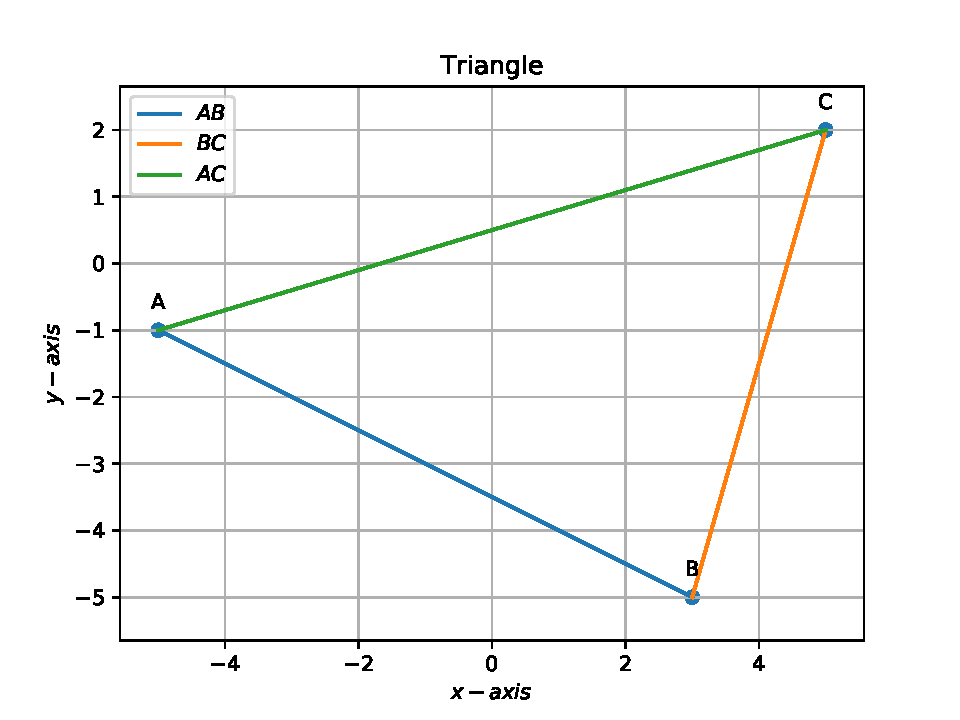
\includegraphics[width=\columnwidth]{./figs/problem1b.pdf}
	\end{center}
\caption{}
\label{fig:Fig2}
\end{figure}
\fi
\end{enumerate}


